% Source: graduate-coursework/Research/How_to_write/00_Contrastive_Synthesis.tex
% Description: \textbf{Rhetorical Genre Studies (Miller, 1984; Bazerman, 1994).

\documentclass[border=4pt]{standalone}
\usepackage{newtxtext,newtxmath}
\usepackage{tikz}
\usetikzlibrary{arrows.meta,positioning,shapes.geometric,calc,decorations.pathreplacing}

\definecolor{garnet}{HTML}{73000A}
\definecolor{atlantic}{HTML}{466A9F}
\definecolor{congaree}{HTML}{1F414D}
\definecolor{horseshoe}{HTML}{65780B}
\definecolor{rose}{HTML}{CC2E40}
\definecolor{honeycomb}{HTML}{A49137}
\definecolor{warmgrey}{HTML}{676156}
\definecolor{black90}{HTML}{363636}
\definecolor{black70}{HTML}{5C5C5C}
\definecolor{black50}{HTML}{A2A2A2}
\definecolor{black30}{HTML}{C7C7C7}
\definecolor{black10}{HTML}{ECECEC}
\definecolor{sandstorm}{HTML}{FFF2E3}

\begin{document}
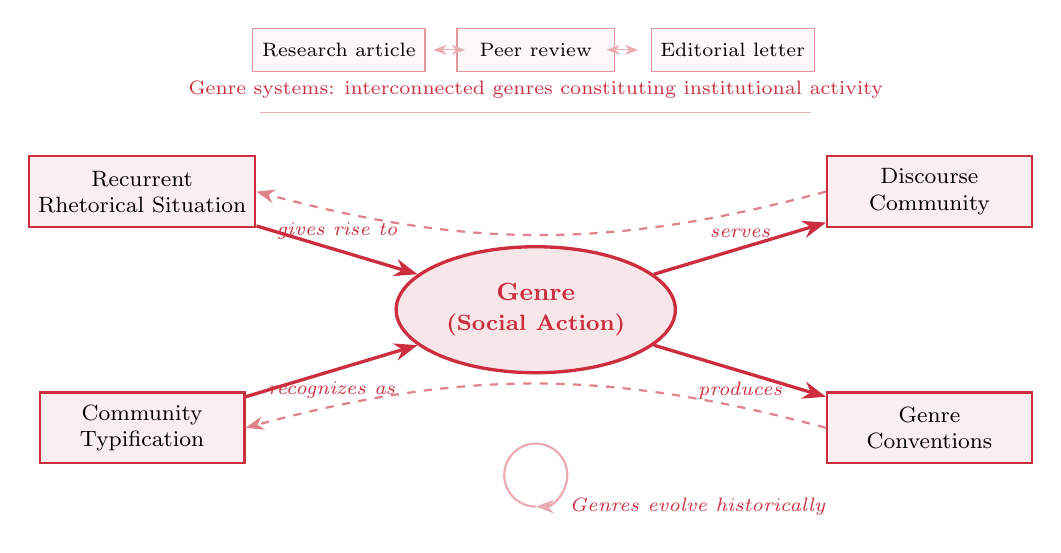
\begin{tikzpicture}[
    every node/.style={font=\footnotesize},
    box/.style={rectangle, draw=rose, thick, fill=rose!8,
        minimum width=2.6cm, minimum height=0.9cm, align=center, font=\footnotesize},
    smallbox/.style={rectangle, draw=rose!50, fill=rose!4,
        minimum width=2cm, minimum height=0.55cm, align=center, font=\scriptsize},
]

% Central concept
\node[ellipse, draw=rose, very thick, fill=rose!12,
    minimum width=3.2cm, minimum height=1.6cm, align=center,
    font=\small\bfseries, text=rose] (genre) at (0,0) {Genre\\{\footnotesize (Social Action)}};

% Recurrent situation
\node[box] (situation) at (-5, 1.5) {Recurrent\\Rhetorical Situation};
\node[box] (typify) at (-5, -1.5) {Community\\Typification};

% Community and conventions
\node[box] (community) at (5, 1.5) {Discourse\\Community};
\node[box] (conventions) at (5, -1.5) {Genre\\Conventions};

% Arrows
\draw[-{Stealth}, very thick, rose] (situation) -- (genre)
    node[midway, above, font=\scriptsize\itshape] {gives rise to};
\draw[-{Stealth}, very thick, rose] (typify) -- (genre)
    node[midway, below, font=\scriptsize\itshape] {recognizes as};
\draw[-{Stealth}, very thick, rose] (genre) -- (community)
    node[midway, above, font=\scriptsize\itshape] {serves};
\draw[-{Stealth}, very thick, rose] (genre) -- (conventions)
    node[midway, below, font=\scriptsize\itshape] {produces};

% Feedback loops
\draw[-{Stealth}, thick, rose!60, dashed] (conventions.west) to[bend right=15] (typify.east);
\draw[-{Stealth}, thick, rose!60, dashed] (community.west) to[bend left=15] (situation.east);

% Dynamic evolution
\draw[-{Stealth}, thick, rose!40] (0, -2.5) arc[start angle=-90, end angle=-450, radius=0.4]
    node[right=0.3cm, font=\scriptsize\itshape, text=rose] {Genres evolve historically};

% Genre system (Bazerman)
\node[font=\scriptsize, text=rose, align=center] at (0, 2.8)
    {Genre systems: interconnected genres constituting institutional activity};
\draw[thin, rose!40] (-3.5, 2.5) -- (3.5, 2.5);

% Examples
\node[smallbox] at (-2.5, 3.3) {Research article};
\node[smallbox] at (0, 3.3) {Peer review};
\node[smallbox] at (2.5, 3.3) {Editorial letter};
\draw[{Stealth}-{Stealth}, thin, rose!40] (-1.3, 3.3) -- (-0.9, 3.3);
\draw[{Stealth}-{Stealth}, thin, rose!40] (0.9, 3.3) -- (1.3, 3.3);

\end{tikzpicture}
\end{document}
